\section{Introduction}

Critical infrastructures are integral to the functioning of our daily lives. They are changing in order to solve different problems it faces nowadays. The growth of power demand, integration of markets and the need of sustainable and efficient energy sources. \\
One such important critical infrastructure is the energy grid. A typical energy grid is divided into several domains such as generation, transmission and distribution. All the actors within domains of a energy grid are connected through information and communication technology(ICT). Hence, energy grids have continuously been the target of cyber attacks and provided their use of standard architecture and internet, they are relatively easier to attack. Security mechanisms have been introduced to protect against such attacks. Security-by-design approach has been used to determine security measures for various systems during design phase. With this approach, the system is equipped to deal with difficult scenarios before deployment. \\ However, there may be instances where the user must intervene to control the system when under attack and stress. During such instances, the user maybe asked to re-authenticate themselves, whereat remembering increasingly difficult passwords and entering correctly actually causes an overhead on the user. The security mechanism in fact is a hindrance here. Such a situation could be avoided if the authentication system in place is usable under different conditions.
%Intro big pic, narrow, Related work seperate subsection

\subsection{Related Work}
Usability of security is an area of research that has been overlooked. More focus is placed on security itself, hence the presence of extensive literature on security in information systems and lack thereof in the case of usability. Smart grid is a vast interconnection of several different kinds of components across several domains. There are several key components that interact with each other that expose several vulnerabilities\cite{liu2012cyber}. There are several vulnerabilities across communication protocols, legacy devices and technologies. Additionally, when designing a system, new vulnerabilities may be found, rendering current security infrastructure weaker. A cyber-physical approach\cite{mo2012cyber} has been presented to tackle new security challenges. They propose a system model uses security requirements and vulnerabilities to identify countermeasures. The HyRim project\cite{scada2014attack} highlights in detail the taxonomy of attacks on SCADA systems and prospective solutions to improve the security.
\newline
There is a lack of usability standards that determine the goals of usability for energy systems. Usability is not directly engineered, but is rather a consequence of system engineering. There are guidelines that aid engineers in developing usable systems\cite{nurse2011guidelines}. Standards such as ISO 9241-11\cite{bevan2015iso} state that usability must be measured in terms of effectiveness, efficiency and satisfaction. These terms must be related to the system of interest using performance metrics of the respective system.A first look at such a relation is provided\cite{kainda2010security}, however is not comprehensive enough to establish a concrete relation between systems. In this paper, we build on this idea to derive a usable security by design approach that begins at the design phase\cite{nielsen1992usability}.

\section{Security in Critical Infrastructure}

The availability of electric power is the primary goal of the power grids. As the smart grid develops, these power systems are more sophisticated, using modern technology allowing better control and reliability. Smart grid will feature a highly interconnected network, opening up the possibility for new vulnerabilities.\\

%\textbf{Virtual Power Plant \& Security Issues}\\

Virtual Power Plant(VPP) is one such infrastructure. A VPP is centralized system that aggregates various energy sources to meet the energy demand of a geographical area. It relies upon software to remotely control, optimize and dispatch Distributed Energy resources(DERs). At the heart of every VPP is the Energy Management System(EMS). The EMS manages power flows in order to minimize the electricity generation costs and avoid loss of energy produced by generators based on renewable energy sources. 

As a result, there may be new and unprecedented attacks on smart grids, including those that exploit zero-day vulnerabilities. Therefore, in such cases when the system is under attack and needs to be controlled by the operator, an existing authentication system(i.e, the existing security mechanism in place), must be usable under stress. Traditional authentication mechanisms are largely based on password based systems. Having a long random password is good advice. It provides a measure of security for guarding access to important information, such as your online banking account. 
Unfortunately, when faced with having to remember several random fifteen character passwords (characters being A to Z, a to z, 0 to 9 and an assortment of other printable characters such as ! @ \# \$ and \%), most users apply a judgement to the value of the information protected by the password and act accordingly.\\
Some accounts may have a relatively weak password, because of the cost of undue information leakage or harm to the owner if the account is compromised. Other accounts might have a stronger password because users don't want their money siphoned off by a cyber-criminal. These are judgements about the perceived value of the information. \\
Passwords are also exceptionally susceptible to dictionary and brute force attacks. Simple passwords can be cracked in seconds and longer passwords that include common words and phrases from literature take up to a week to be cracked. Passwords can be called secure if the time required to crack is sufficiently long, such as in years or decades. Such passwords may be constructed from a combination of alphabets, numbers and symbols. There is a trade off though, as such passwords are harder to remember and also hard to enter into a system without errors. It is also compounded by the fact that users are recommended to change passwords periodically. This invites a lot of pressure onto users who are not technologically friendly and are oblivious to the system structure. Additionally, in certain circumstances, such as an emergency situation, a user may need quick access to resources. In such a situation, a user is more likely to make mistakes entering a complicated password and being denied access. If the user is an operator of a smart grid, this could lead to a catastrophe. Therefore, the most secure passwords are, in fact, the least usable. 

\smallskip

Therefore, with usability and security being a trade-off, organizations often prioritize security over usability. Hence, to bridge this gap between the two, a framework is required. A framework which can unite the two and allow a system to be secure as well as usable. In the next section, we look towards such a usable security framework.

\section{Usability}

Usability is a measure of the interactive user experience associated with a user interface, such as a website or software application. A user-friendly interface design is easy-to-learn, supports users' tasks and goals efficiently and effectively, and is satisfying and engaging to use.\\

An interface's level of usability can be measured by inviting intended users of the system to participate in a usability testing session. During a usability test session, a user is given a series of tasks to complete by using the system in question, without any assistance from the researcher. The researcher records user behaviours, emotional reactions, and the user's performance as they attempt to accomplish each task. The researcher takes note of any moments of confusion or frustration that the user experienced while trying to complete a task and also tracks whether or not the user was able to satisfactorily complete each task. Analysis of data from several users provides User Experience Engineers a means of recommending how and where to re-design the interface in order to improve its level of usability and thus, the user experience in general.

\smallskip

Usability is the ease of use of a software by any individual in any situation to achieve certain objectives with efficiency. This software, developed by experts, must be usable by any other person effectively. Therefore, the software will have to be developed with a user-centered approach. "Ease of Use" encapsulates the following terms:

\begin{itemize}

\item Effective: Effectiveness is the completeness and accuracy with which users achieve specified goals. It is determined by looking at whether the user's goals were met successfully and whether all work is correct.

\item Efficient: Efficiency can be described as the speed (with accuracy) in which users can complete the tasks for which they use the product. ISO 9241 defines efficiency as the total resources expended in a task. Efficiency metrics include the number of clicks or keystrokes required or the total "time on task".

\item Satisfaction: The comfort and acceptability of use. Additionally, the following two are also considered,

\item Error Tolerant: The ultimate goal is a system which has no errors. But, product developers are human, and computer systems are far from perfect, so errors may occur. An error tolerant program is designed to prevent errors caused by the user's interaction and to help the user in recovering from any errors that do occur.

\item Easy to Learn: An interface which is easy to learn allows users to build on their knowledge without deliberate effort. This goes beyond a general helpfulness to include built-in instruction for difficult or advanced tasks, access to just-in-time training elements, connections to domain knowledge bases which are critical to effective use.

\end{itemize}

Usability depends on a number of factors including how well the functionality fits the user needs, how well the flow through the application fits user tasks and how well the response of the application fits user expectations. We can learn to be better user interface designers by learning design principles and design guidelines. But even the most insightful designer can only create a highly-usable system through a process that involves getting information from people who actually use the system. Usability is the quality of a system that makes it easy to learn, easy to use, easy to remember, error tolerant, and subjectively pleasing.

\smallskip

From the user's perspective, usability is important because it can make the difference between performing a task accurately and completely or not, and enjoy the process or be frustrated. From the developer's perspective, usability is important because it can mean the difference between the success or failure of a system. From a management point of view, software with poor usability can reduce the productivity of the workforce to a level of performance worse than without the system. In all cases, lack of usability can cost time and effort and can greatly determine the success or failure of a system. Given a choice, people tend to buy systems that are more user-friendly.

\smallskip

The key principle for maximizing usability is to employ iterative design, which progressively refines the design through evaluation from the early stages of design. The evaluation steps enable the designers and developers to incorporate user and client feedback until the system reaches an acceptable level of usability.\\

The preferred method for ensuring usability is to test actual users on a working system. Achieving a high level of usability requires focusing design efforts on the intended end-user of the system. There are many ways to determine who the primary users are, how they work, and what tasks they must accomplish. However, clients' schedules and budgets can sometimes prevent this ideal approach. Some alternative methods include user testing on system prototypes, a usability audit conducted by experts, and cognitive modelling.

\smallskip

Usability is one of the focuses of the fields of Human Factors Psychology and Human-Computer Interaction. As the name suggests, usability has to do with bridging the gap between people and machines. A user interface (or human-computer interface) refers to the parts of a hardware and/or software system that allows a person to communicate with it. This includes output devices (the way the computer communicates with a user) and input devices (the way a user communicates with the computer). Typical "output devices" include computer monitors and the operating systems that run on them, and also include speakers and other devices that provide feedback. "Input devices" include peripherals like keyboards, mice, and joysticks, and also include microphones and eye movement devices. Each of these interface components has devices corresponding to the visual (sight), aural (sound), and haptic(touch) channels of the brain. Usability engineering studies these elements of the user's experience.

\subsection{Usability Standards: ISO 9241}

ISO 9241 is a multi-part standard from the International Organization for Standardization(ISO) covering ergonomics of human-computer interaction. It is managed by the ISO Technical Committee 159. Part 1 is a general introduction to the rest of the standard. Part 2 addresses task design for working with computer systems. Parts 3-9 deal with physical characteristics of computer equipment. Part 110 and parts 11-19 deal with usability aspects of software, including Part 110 (a general set of usability heuristics for the design of different types of dialogue) and Part 11(general guidance on the specification and measurement of usability). \\

The ISO 9241-11 standard defines usability as "the extent to which a product can be used
by specified users to achieve specified goals with effectiveness, efficiency and satisfaction
in a specified context of use". This definition clearly states that usability is not a single,
one-dimensional property but rather a combination of factors.
The ISO/IEC 9126-4 Metrics recommends that usability metrics should include:
\begin{itemize}
\item Effectiveness: The accuracy and completeness with which users achieve specified
goals.

\item Efficiency: The resources expended in relation to the accuracy and completeness
with which users achieve goals.

\item Satisfaction: The comfort and acceptability of use.
\end{itemize}

However, the actual ways of how these should be measured are very often left at the
discretion of the evaluator. Therefore, we need to establish these metrics. To a normal
person without technical knowledge, usability is measured by the ease of use of a system in a
particular situation. But when designing and implementing a system, the engineers and
developers involved need to measure the usability using metrics. In the coming sections, we attempt to
establish grounds for deriving these metrics.

\medskip

ISO 9241-11 also emphasises that usability is dependent on the context of use and that the
level of usability achieved will depend on the specific circumstances in which a product is
used. The context of use consists of the users, tasks, equipment (hardware, software and
materials), and the physical and organisational environments which may all influence the
usability of a product (see \ref{fig:usability1}).

\begin{figure}[H]
\caption{Usability Framework. Source: \cite{bevan1995human}}
\label{fig:usability1}
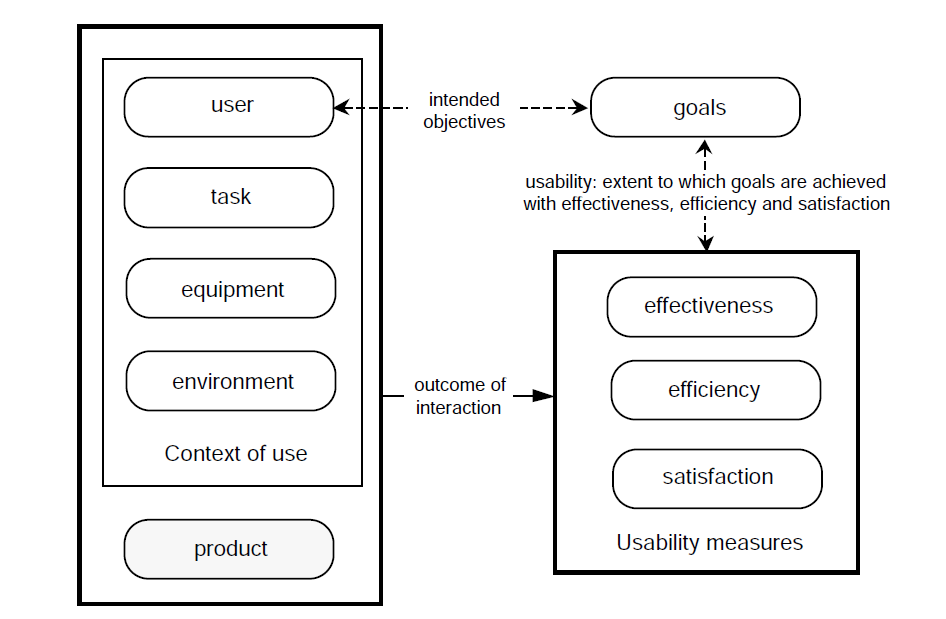
\includegraphics[scale=0.2]{img/usability1.png}
\end{figure} 

ISO 9241-11 describes how the usability of a product can be defined, documented and
verified as part of a quality system which conforms to ISO 9001 (Figure \ref{fig:usability2}). The overall
context of use should be identified, usability requirements should be specified, usability issues
should be monitored during development, and the usability achieved should be evaluated. \\
Dealing with usability as part of a quality system for design and development of products,
as specified in ISO 9001, involves the systematic identification of requirements for usability,
including usability measures and verifiable descriptions of the context of use. These provide
design targets which can be the basis for verification of the resulting design.
ISO 9001 specifies what is required for a quality system. A quality system is a
documented set of procedures intended to ensure that a product will meet initially stated
requirements. A quality system is a desirable (though not sufficient) condition for achieving the 
quality of the end product. 

\begin{figure}[H]
\caption{Quality Plan. Source: \cite{bevan1995human}}
\label{fig:usability2}
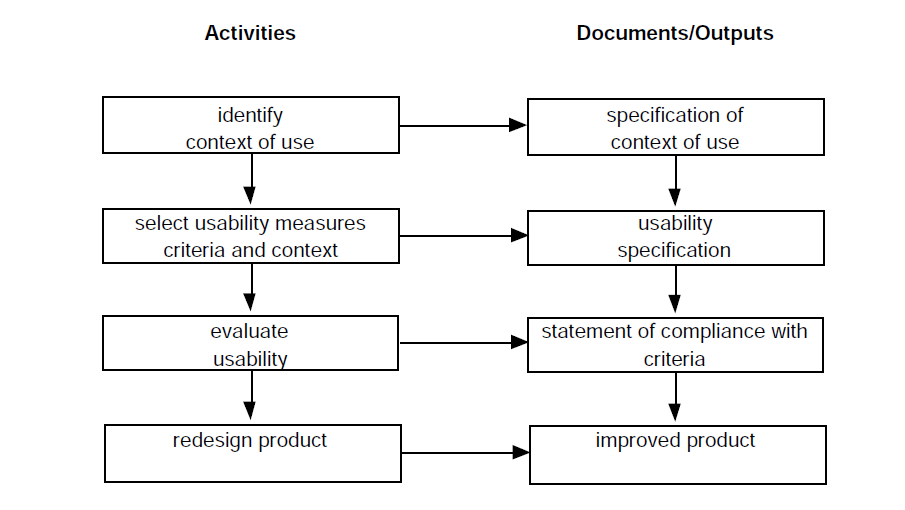
\includegraphics[scale=0.2]{img/usability2.png}
\end{figure} 

\textbf{Usability requirements:} Prior to the development of a custom system, the purchasing
organisation should specify the usability requirements which the system must meet and
against which acceptance testing may be carried out. Specific contexts in which usability is to
be measured should be identified, measures of effectiveness, efficiency and satisfaction
selected, and acceptance criteria based on these measures established. \\
\textbf{Monitor usability:} At various stages during the development process the developer should
measure the usability achieved against these targets. This information enables objective
decisions to be taken about the need for design changes to enhance usability, and about trade-offs
which may be appropriate between usability and other requirements. \\
\textbf{Usability evaluation:} The characteristics of the context in which a product is likely to be
used need to be identified. To ensure the validity of test results the users, tasks and
environments used for the evaluation should match the real context of use as closely as
possible.


\section{Framework for Usable Security}
Since, usability and security are normally at opposite ends of the spectrum, there are no uniform set of criteria or guidelines that define a usable security system. Nurse et al\cite{nurse2011guidelines} 
compiled a list as guidelines for usable security.
\newline
To design a security system that is usable, we need appropriate metrics to measure its efficiency. Therefore, we need to define such metrics. With the security system in focus, the usability metrics must stem from the properties of security themselves. Through this process, we then develop a security with a view of usability in the design stage itself, rather than first building a security system and then attempting to incorporate usability. When designing a security system, each component of security, every module could be tested for its usability wherever applicable. Usability of one component may affect that of another. That is, if a component is less usable, the overall usability of the system reduces, since the user may spend more resources on such a component at the cost of others. In other words, it hinders the performance of the system as a whole. The issue at hand is that due to the lack of usability metrics or any quantifiable value, any system cannot yet be defined as usable or unusable. \\


Quality in Use Integrated Measurement(QUIM)\cite{seffah2001quim} was proposed to primarily address these issues by aggregating usability standards, metrics and methods from numerous sources in one centralized knowledge base. QUIM is a repository of 10 factors, 26 criteria, and 128 metrics for assessing usability/quality in use of software systems. Most of the existing usability models/standards may be seen as specific instances of the QUIM model. \\

Usability of a system, though determined by efficiency, effectiveness and satisfaction, is still not quantified. Furthermore, the three properties can be measured in various ways for different systems. To specialize usability for a security system, a relation between security and usability must be established. In the presence of such a relation, a security system's properties can be optimized, via metrics, such that usability properties are satisfied. This method can be used to integrate usability into any system instead of security systems. \\ 

In essence, each property has a metric with a desirable value that makes the system usable.
But these metrics are defined when a system operates in normal mode. When in any situation
other than normal mode, these metrics may vary and the system will have to adapt to the
situation. This variation could be used as an indication of how usable the system is.

A security system will have to go through a usability engineering cycle subject to constraints
and metrics. Ideally, security must not be an extra design layer, but it should be included in
the whole software design process of the systems used in grids. This may be particularly
hard to achieve, since smart grids at the moment use common operating systems(Windows,
linux), and therefore leaves this question open. It might be possible to develop these
common OSes with respect to the security required for smart grids, though this does not
appear to be considered as yet. Similarly, usability must be considered in the design phase as well. Individual components may be evaluated for usability. This may be considered as \textbf{Usable Security by Design.}


\subsection{Methodology}
With respect to the smart grid, the asset we are trying to protect is the control and information flow of the grid. Therefore, being a critical infrastructure, their estimated value is evidently high.   
\newline The countermeasure, in this case, is an authentication system. To move forward with the framework, 	we need to identify the elements of the authentication system. Generally, they contain: An interface, a database, an authentication protocol run, key/token management and encryption algorithms. All the elements of the system can be measured using suitable metrics to quantify their impact on the usability of the system. In table \ref{tab:security-usability-relation}, different properties or factors affecting security are listed. The third column contains these factors, the second column contains the criteria for usability, which also represent the requirements for usability in this case and the first column contains the properties and factors affecting usability. The table is arranged such that if the security factors are optimized, they either directly satisfy the usability factors(or properties) in the first column or they satisfy the usability criteria(in the second column) and transitively satisfying the usability factors(or properties). 


\begin{center}
\begin{table}[H]
\caption{Relation between security and usability}
\label{tab:security-usability-relation}
\resizebox{9cm}{!}{
\begin{tabular}{|c|c|c|} 
\hline
\multicolumn{2}{| c |}{\textbf{Usability}}
& \textbf{Security} \\
\hline
\textbf{Factors and Properties} & \textbf{Criteria/Requirements} & \textbf{Factors and Properties} \\
\hline
Effectiveness & Accuracy & EER, Accuracy \\
\hline
Efficiency & Minimal Action & \makecell{Task Completion Time, \\ Monetary cost of performing the task} \\
\hline
{Satisfaction} & {Operability, Minimal Action} &  {Interface Design} \\
\hline
Productivity & Memory Load & Authentication Token \\
\hline
Learnability & \makecell{Time to learn functionalities,\\ Minimal Action} &  Interface Design \\
\hline
\end{tabular}
}
\end{table}
\end{center}


The second column in table \ref{tab:security-usability-relation} specifies the requirements(or criteria) for usability of a security system. These criteria were specifically selected for a scenario involving a user attempting to gain access through an authentication mechanism. These requirements need to be quantified with metrics for an evaluation. the table \ref{tab:possible-values} shows the metrics and the desired values for this specific use case.

\begin{center}
\begin{table}[H]
\caption{Possible values for metrics}
\label{tab:possible-values}
\resizebox{9cm}{!}{
\begin{tabular}{|c|c|}
\hline
\textbf{Security Metric} & \textbf{Permissible Range} \\
\hline
EER & As low as possible, tending to 0\\
\hline
Accuracy (Success Rate of Correct Input) & ~100\%. \\
\hline
Task Completion Time & Time in seconds; Depends on use case \\
\hline
Interface Design & User rating based on satisfaction and feedback\\
\hline
Memory Load & User rating based on satisfaction and feedback\\
\hline
\end{tabular}
}
\end{table}
\end{center}

Therefore, a \textit{usable security framework for an authentication system} consists of an authentication system which includes a user-friendly interface, requires a user to have little to no authentication tokens, satisfies the criteria for a conventional security system such as Confidentiality, Integrity and Availability in addition to all the criteria mentioned above. The evaluation of these criteria with respect to their metrics should fall in the permissible zone. The user also must provide feedback and specify the drawbacks, if any and suggestions to improve the system from the perspective of usability. 

\subsection{Using The Framework}
To use the usable security framework, the organization intending to use it has to specify the goals on the system. Similar systems may be optimized in different ways, hence the developers need to specify the priorities. The important factors and properties affecting the system must be listed and with respect to the priorities, i.e, goals of the system and the developers, those factors affecting the user most should be selected. For example, let the goal be a highly efficient authentication mechanism. Therefore, accuracy is a goal and a priority.\\
The usability framework, with the help of QUIM, breaks down usability factors into criteria that can be quantified. Those usability factors that are of importance to the developers must be focused upon, however, the three usability factors, efficiency, effectiveness and satisfaction must all be used to satisfy usability, as per ISO 9241-11. In our example, accuracy of the system will be the focus and hence it will need to be optimized.\\
In the next step, those factors derived from the target system must be used as quantifiable values to measure the criteria specified in table \ref{tab:security-usability-relation}. If a criteria cannot be quantified, alternative criteria can be selected from the QUIM usability criteria. In any case, the prioritized factors must be quantified. In our example, accuracy is a measurable quantity of the system as well as the usability criteria used to determine the efficiency.\\
Accordingly, the factors measured from the system must be used to quantify the usability criteria, which help measure the usability factors. 

\subsection{Validation}
To demonstrate how this framework could be used, we use an example. Two different authentication systems were tested, a fingerprint matching system and a simple password system. The evaluation involved participants using both types of systems and then answering a questionnaire. To assess fingerprint matching, two approaches were used. Since, there are several types of fingerprint matching algorithms, performance may vary. Therefore the most common implementations found in real life was used. First, an optical scanner of fingerprints was evaluated. An optical scanner scans the fingerprint into an optical image and compares the image as is with a database of images. This process is slow and less secure, as images of fingerprints are stored unprotected in the database. The second kind was a capacitive scanner, where fingerprints are read using varying electric charges when a ridge comes in contact with the scanner. This change is charge is converted to digital data, which is then analysed to look for unique features. Data is stored digitally, though not necessarily encrypted. This form of storing data is still vulnerable but more secure than images. There were 30 participants whose fingerprints were added to a database of more than 1000 entries. The results of the capacitive scanner were found to be more optimal. They are shown below:

\begin{center}
\begin{table}[H]
\caption{Results for Biometric systems.}
\label{tab:result2}
\resizebox{9cm}{!}{
\begin{tabular}{|c|c|}
\hline
\textbf{Security Metric} & \textbf{Observed values} \\
\hline
EER & 3.9\%\\
\hline
Accuracy (Success Rate of Correct Input) & 96.1\%. \\
\hline
Task Completion Time & Average of 1.8 seconds \\
\hline
Interface Design & 4.2\\
\hline
Memory Load & 5\\
\hline
\end{tabular}
}
\end{table}
\end{center}

The EER and Accuracy values claimed were 1.9\% and 98.1\% respectively by the algorithm. The fingerprint matching was not developed in-house but was rather off the shelf for assessment. Possible reason for the lower values is the smaller sample space. The values shown against "Interface Design" and "Memory Load" are mean values of the scores given by participants. The scores were based on a scale from 1 to 5, where 1 represents "Very Uncomfortable" to "Very Comfortable".\\
Shown below is the inference table for password systems. Typical password systems include the user presenting a username and password, both entered by the user. The same setup was used for the following evaluation. Users were registered with a simple password system and then were asked to login. Standard password recommendations were used, such as using passphrases, combinations of letters, both uppercase and lowercase, numbers and symbols. 

\begin{center}
\begin{table}[H]
\caption{Inference Table for password based systems.}
\label{tab:infer_password}
\resizebox{9cm}{!}{
\begin{tabular}{|c|c|c|}
\hline
\textbf{Security Metric} & \textbf{Expected values} & \textbf{Observed values} \\
\hline
Accuracy (Success Rate of Correct Input) & 100\% & 100\%. \\
\hline
Task Completion Time & 10-12 seconds & Avg of 12.2 seconds \\
\hline
Interface Design & >4 & 4.7\\
\hline
Memory Load & >4 & 3.5\\
\hline
\end{tabular}
}
\end{table}
\end{center}

Interface Design and Memory Load were scored with the same method as for biometric systems. Interface design received a higher score due to the familiarity to users, however due to complicated passwords, it was harder to remember multiple difficult and complex passwords for various systems simultaneously. It also affected the task completion time, which was relatively longer. Accuracy is 100\% since a correctly entered password was never rejected. We are not counting mistyped passwords. A reason for this is, the measure used for biometrics is accuracy. In biometric systems fingerprints are rarely falsely entered, although a possibility. Users are aware of which fingerprint is required. Therefore, in fingerprint systems accuracy of the algorithm is used as a measure for the performance. To keep the consistency, accuracy was used for password systems.

\subsection{Inference}


\subsection{Integration into SDL}
How to assess usability in SDL?

\section{Conclusion}


